% !TEX encoding = UTF-8
% !TEX TS-program = pdflatex
% !TEX root = data mining.tex
% !TEX spellcheck = it-IT
\section{Gestione degli outliers}\label{gestione-degli-outliers}

I risultati ottenuti con il terzo modello sono molto buoni, ma osservando la distribuzione dei campioni si possono notare dei punti che escono dalla distribuzione.

\begin{figure}[htbp]
	\centering
	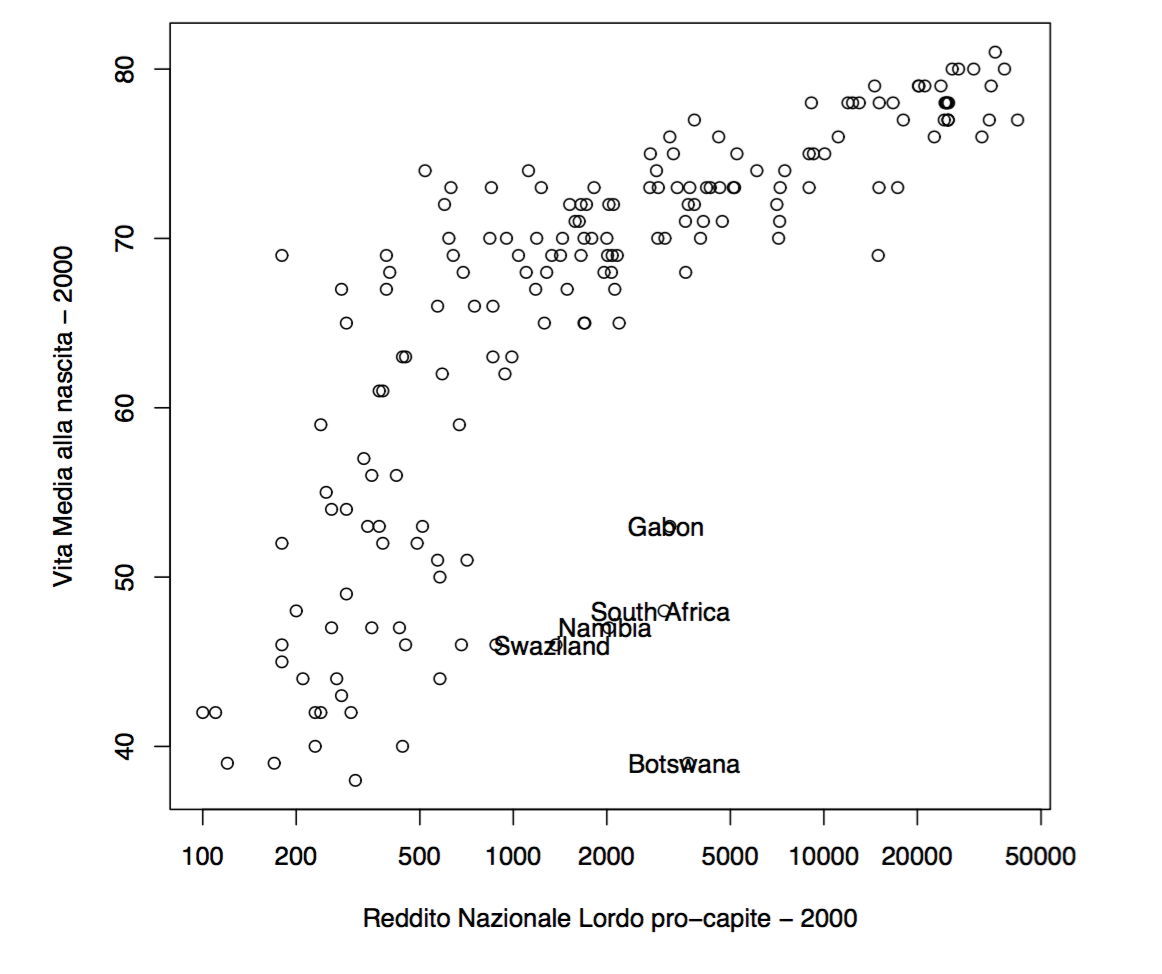
\includegraphics[width=.5\textwidth]{./notes/immagini/l8-fig1.png}
\end{figure}

Questi stati che si discostano sono principalmente africani e si può pensare che il comportamento diverso sia causato dalle loro condizioni socio-economiche, come l'AIDS che abbassa l'aspettativa di vita o il petrolio che aumentare la ricchezza solamente di poche persone.

Si può quindi pensare di calcolare il modello senza utilizzare questi outliers.

\begin{verbatim}
lm(formula = elf.5 ~ logGNI, data = elf.out1.data)
Residuals:
Min        1Q       Median      3Q        Max
-1.111e+09 -2.880e+08 -3.471e+07 2.817e+08 1.298e+09
Coefficients:
Estimate Std. Error t value Pr(>|t|) 
(Intercept) -2.344e+09 1.587e+08 -14.77 <2e-16 *** 
logGNI 5.221e+08 2.059e+07 25.36 <2e-16 ***
---
Signif. codes: 0 ‘***’ 0.001 ‘**’ 0.01 ‘*’ 0.05 ‘.’ 0.1 ‘ ’ 1
Residual standard error: 423200000 on 166 degrees of freedom 
Multiple R-Squared: 0.7948, Adjusted R-squared: 0.7935 
F-statistic: 642.9 on 1 and 166 DF, p-value: < 2.2e-16
\end{verbatim}
\begin{figure}[htbp]
	\centering
	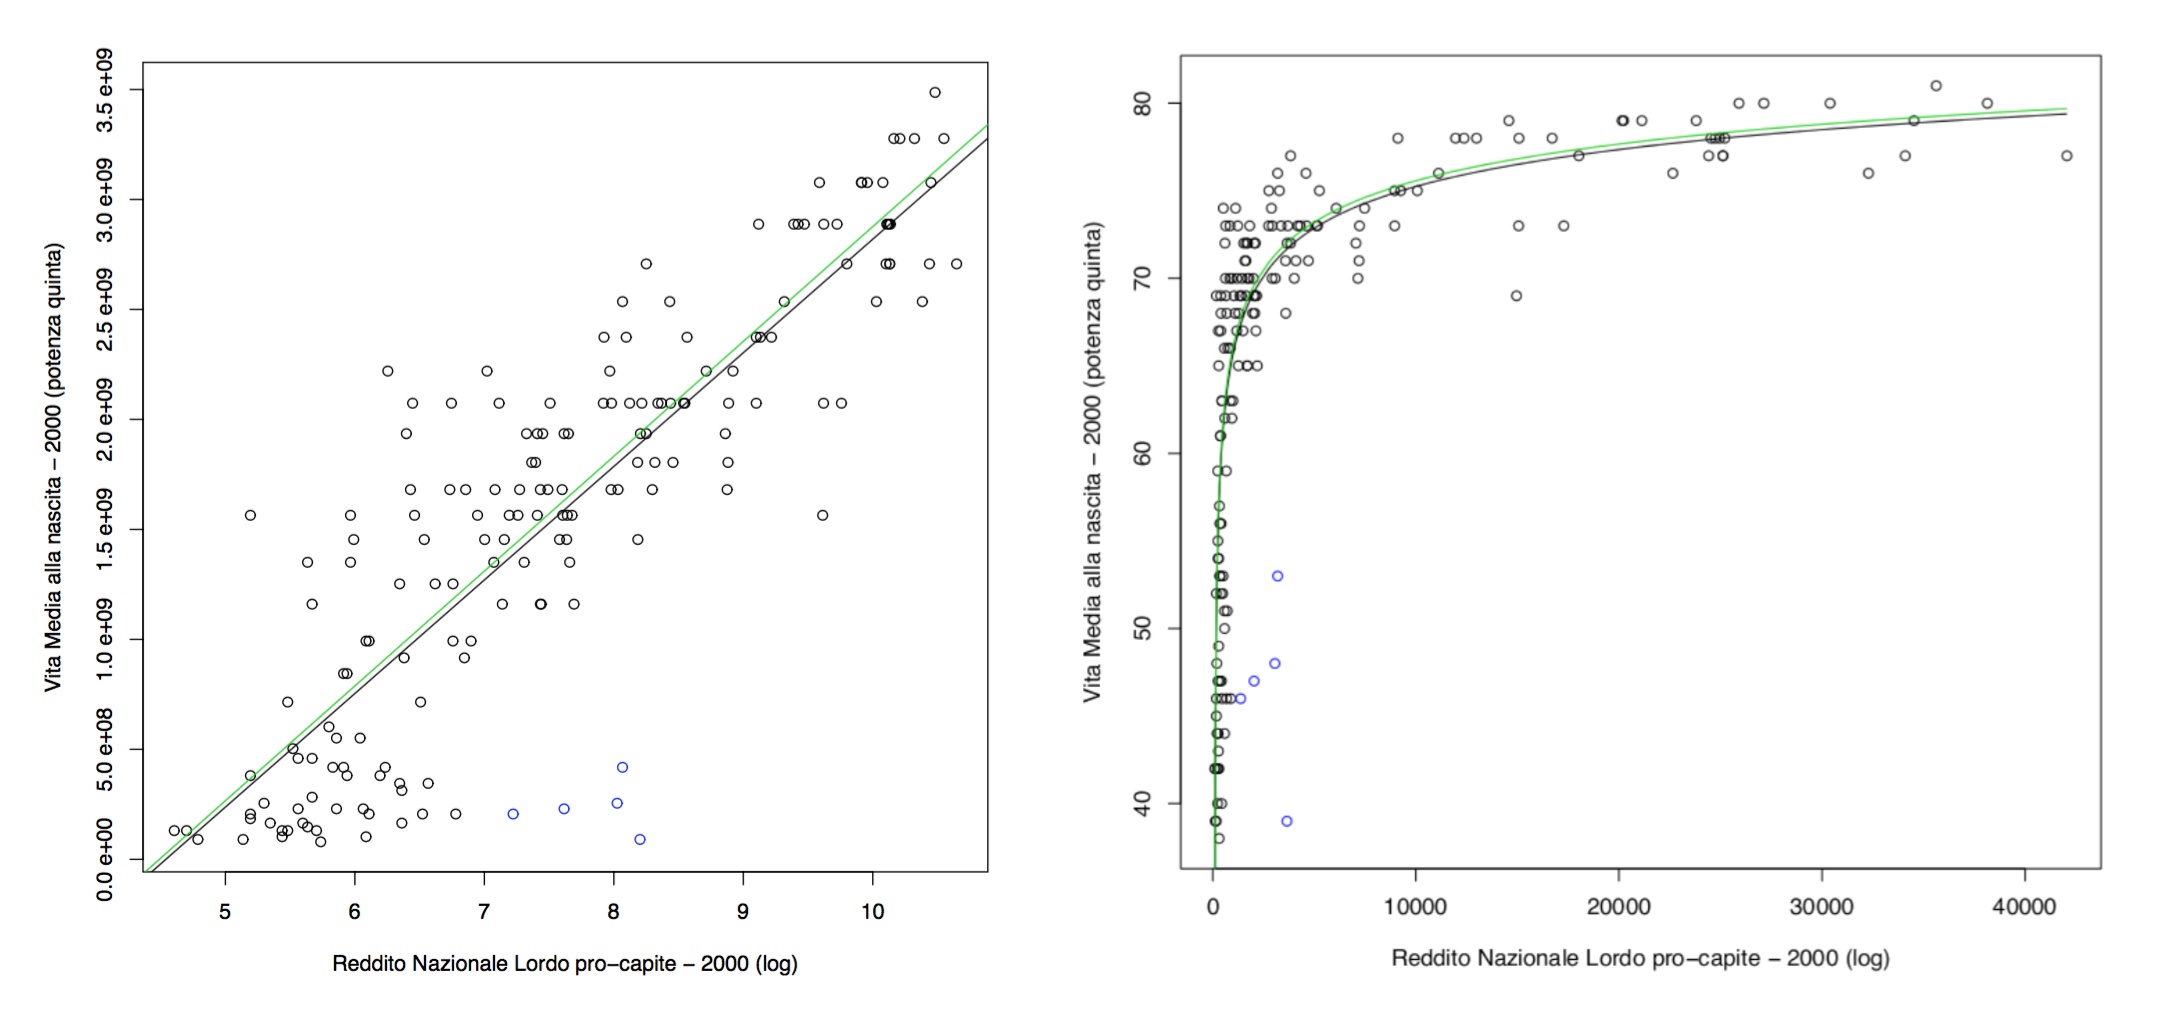
\includegraphics[width=1\textwidth]{./notes/immagini/l8-fig2.png}
	\caption{In verde il nuovo modello senza outliers, in nero il terzo modello. Si può notare che il nuovo modello è traslato verso l'alto perché non considera gli outliers (punti in blu)}
\end{figure}

In modo simile a come effettuati prima si può calcolare la varianza residua su scala originale, considera \textbf{solo} le osservazioni usate per la stima, ottenendo così una riduzione del $ 26\% $.

\begin{figure}[htbp]
	\centering
	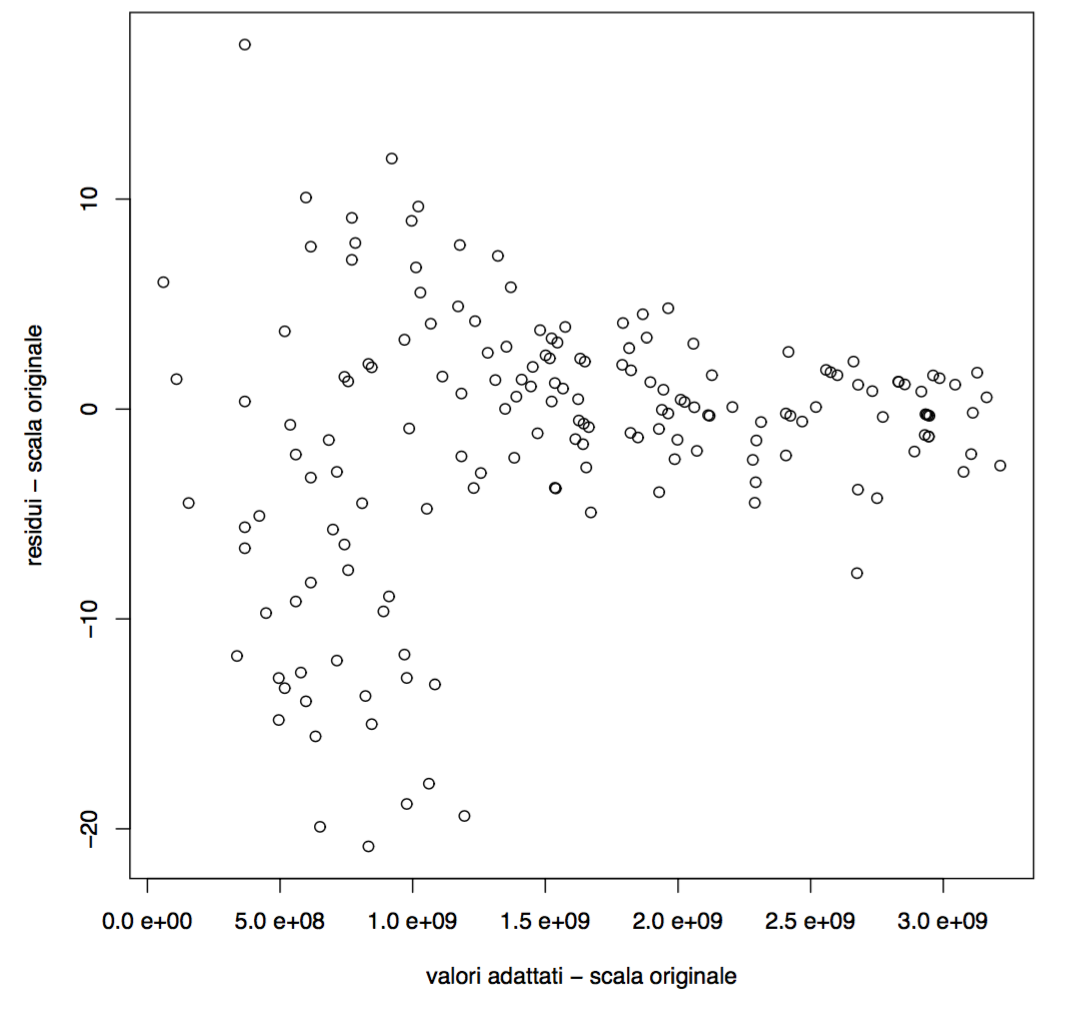
\includegraphics[width=.5\textwidth]{./notes/immagini/l8-fig3.png}
	\caption{In residui nella scala originale. Quando l'ipotesi di indipendenza non è del tutto soddisfatta conviene effettuare una trasformazione della variabile risposta.}
\end{figure}


\chapter{Modello lineare con più variabili esplicative}

\textbf{Dataset delle scuole}: è ragionevole pensare che la quantità di
soldi disponibili per una scuola sia una misura della qualità
dell'insegnamento?

Variabili a disposizione:

\begin{itemize}
\item
  Spese medie annuali per studente
\item
  rapporto studenti/insegnanti
\item
  salario medio annuale
\item
  percentuale di studenti che hanno effettuato il test SAT
\item
  punteggio medio totale (per stato)
\item
  punteggio per le materie verbali)
\item
  punteggio per le materie matematiche
\end{itemize}

\begin{figure}[htbp]
	\centering
	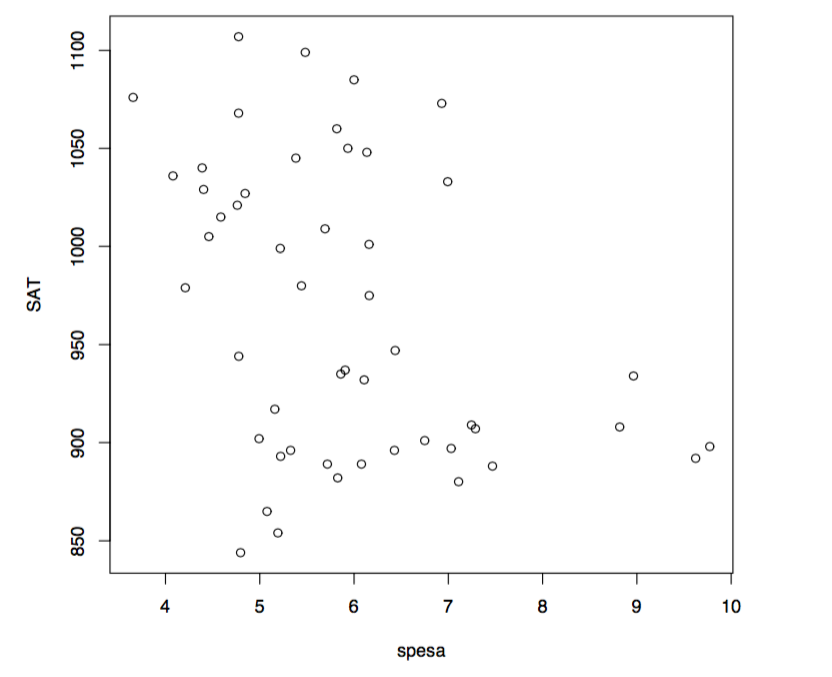
\includegraphics[width=.5\textwidth]{./notes/immagini/l8-fig4.png}
	\caption{Diagramma di dispersione \textit{spesa - SAT}}
\end{figure}

Per la distribuzione dei dati è possibile utilizzare la correlazione di \textbf{Bravais-Pearson}

$$
\rho = \frac{cov(x,y)}{\sqrt{var(x)var(y)}}
$$

il quale risulta essere -0.381 con \textit{p-value} 0.006, quindi sembra che ci sia una correlazione lineare negativa tra le due variabili.

Per verificare ciò è possibile utilizzare il modello di regressione semplice

$$
\text{SAT} = \alpha + \beta \text{SPESA} + \epsilon
$$

Ottenendo $ \hat{\alpha} = 1089.294 $ e $ \hat{\beta} = -20.892 $ con \textit{p-value} = 0.0064, quindi con i dati estremamente contrari all'ipotesi nulla.

\textbf{\textit{p-value}} = probabilità di osservare un valore maggiore di $ t_{oss} $ rispetto la \textit{t} di Student. In questo caso $ t_{oss} = -2.85 $.

Da questo primo modello emerge quindi che c'è una correlazione lineare tra queste due variabili, ma che l'aumento della spesa per l'istruzione porta ad una diminuzione della valutazione SAT, il che sembra contro intuitivo.

\section{Correlazione parziale}

Tra i dati a disposizione c'è anche la percentuale di studenti che si sono sottoposti al SAT e come si può notare dal grafico questa percentuale varia molto di stato in stato.
Questo perché dall'esito del SAT dipende l'ammissione nelle università statali più prestigiose, mentre per altre università è possibile fare altri test.
Morale della favola: negli stati con una percentuale di test effettuati minore l'esito medio è più alto perché lo fanno solo i secchioni.

Sarebbe bello poter definire un modello che tenga conto anche di questa correlazione.

\begin{figure}[htbp]
	\centering
	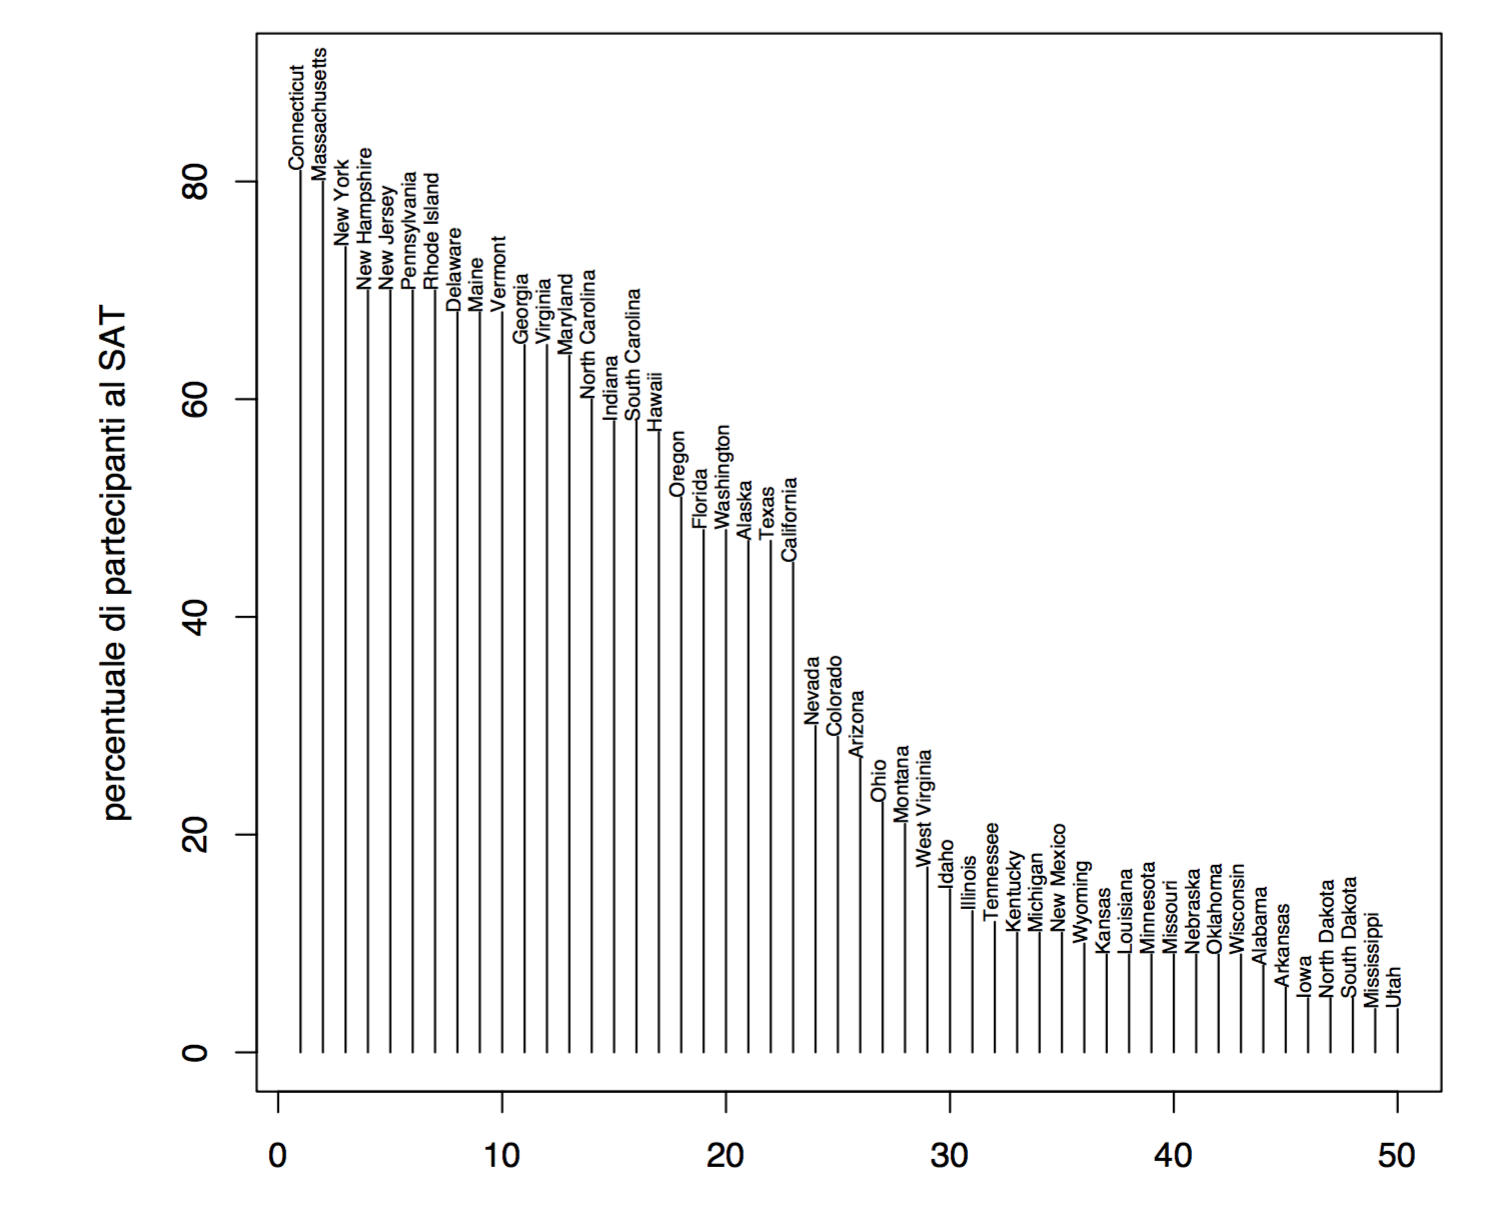
\includegraphics[width=.5\textwidth]{./notes/immagini/l8-fig5.png}
	\caption{Percentuale di studenti che si sottopongo al SAT per stato}
\end{figure}

\begin{figure}[htbp]
	\centering
	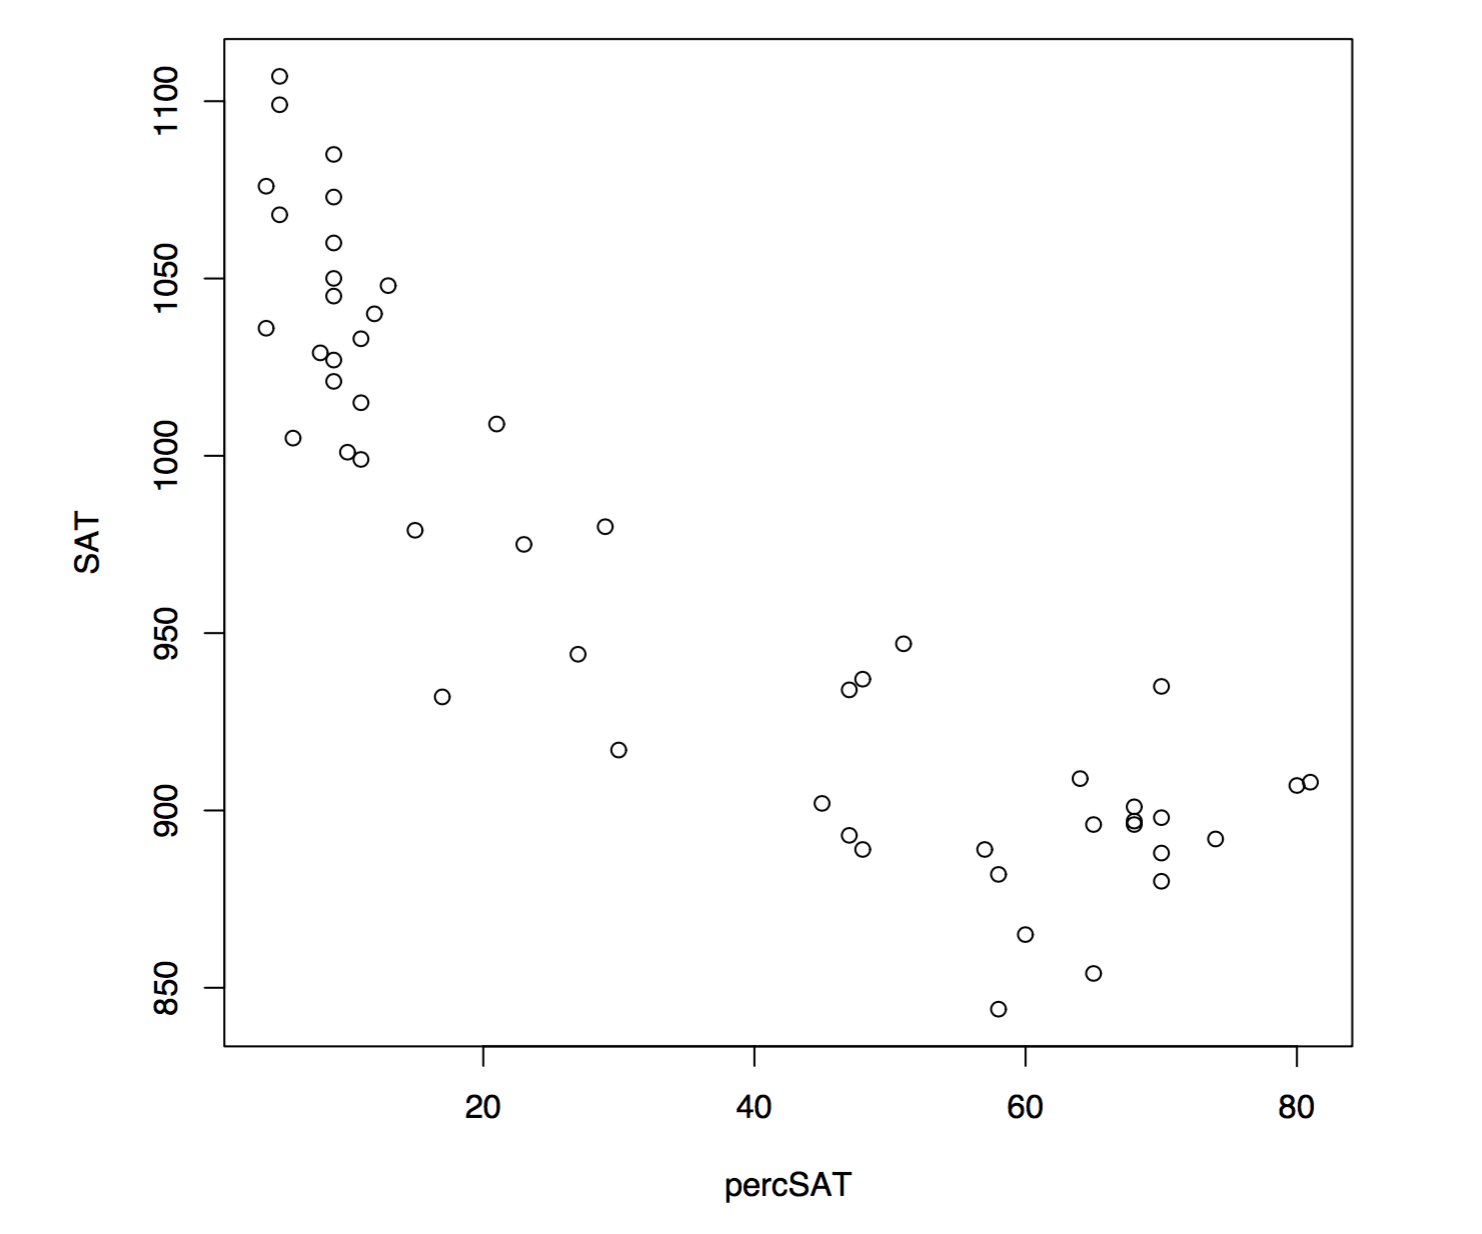
\includegraphics[width=.5\textwidth]{./notes/immagini/l8-fig6.png}
	\caption{Diagramma di dispersione \textit{perSAT - SAT}}
\end{figure}

Una formulazione più generale di questo problema riguarda una variabile di risposta \textit{Y} e almeno una variabile esplicativa $ X_1$. \`{E} poi presente almeno un'altra variabile $ X_2 $ che potenzialmente influenza sia $ X_1 $ che $ Y $.

Se c'è questa influenza, il coefficiente di correlazione $ \rho $ fornisce delle indicazioni errate in quanto $ X_2 $ ha un'effetto (assunto lineare) sulle altre variabili.

\subsubsection{Il coefficiente di correlazione parziale}

Si vuole stimare l'effetto lineare di $ X_2 $ sulle variabili di interesse.

Come prima cosa vengono calcolati i modelli

\begin{align*}
	Y &= \alpha_0 + \alpha_1 X_2 + \epsilon_Y \\
	X_1 &= \beta_0 + \beta_1 X_2 + \epsilon_{X_1}
\end{align*}

con le solite ipotesi riguardo le distribuzioni degli errori.

Una volta ottenuti i modelli è possibile calcolare i residui, i quali misurano quanto della variabile \textit{Y} e $ X_1 $ rispettivamente non è spiegato dalla variabile $ X_2 $.

\begin{align*}
Z_{Y} &= Y - \alpha_0 - \alpha_1 X_2 \\
Z_{X_1} &= X_1 - \beta_0 - \beta_1 X_2
\end{align*}

Con queste due nuove variabili è possibile calcolare il \textbf{coefficiente di correlazione parziale} tra $ Y $ e $ X_1 $ al netto dell'effetto lineare di $ X_2 $.

$$
\rho_{YX_1:X_2} = \frac{cov(Z_Y, Z_{X_1})}{\sqrt{var(Z_Y)} \sqrt{var(Z_{X_1})}}
$$

Calcolando questo coefficiente per il data set di riferimento si ottiene 0.391, ovvero il segno della correlazione tra \textit{SAT} e \textit{SPESA} è cambiato. 

\subsubsection{Stima del nuovo modello}

$$
\text{SAT} = \beta_0 + \beta_1\text{SPESA}+\beta_2\text{PERC\_SAT} + \epsilon
$$

Questo modello dovrebbe cogliere l'effetto congiunto delle due variabili, fornendo una misura di quanto ciascuna delle due variabili influisce singolarmente su \textit{SAT}.

La stima viene fatta ai minimi quadrati, utilizzando la versione più generale del modello

$$
Y = \beta_0 + \beta_1 X_1+\beta_2X_2 + \epsilon
$$

Si tratta quindi di stimare i coefficienti $ \hat{beta}_0, \hat{beta}_1 $ e $ \hat{beta}_2 $ in modo tale che

\begin{align*}
y_1 &\approx \hat{\beta}_0 + \hat{\beta}_1 x_{1,1}+\hat{\beta}_2 x_{2,1}+ \epsilon\\
y_2 &\approx \hat{\beta}_0 + \hat{\beta}_1 x_{1,2}+\hat{\beta}_2 x_{2,2}+ \epsilon\\
\vdots
y_n &\approx \hat{\beta}_0 + \hat{\beta}_1 x_{1,n}+\hat{\beta}_2 x_{2,n}+ \epsilon\\
\end{align*}

$$
s^2(\beta_0, \beta_1, \beta_2) = \sum\limits_{i=1}^n(y_i - \beta_0 + \beta_1 x_{1,i}+\beta_2 x_{2,i} )
$$

scegliendo $ \hat{beta}_0, \hat{beta}_1 $ e $ \hat{beta}_2 $ in modo da minimizzare $ s^2 $.

$$
s^2(\hat{\beta}_0 , \hat{\beta}_1 , \hat{\beta}_2) \leq s^2(\beta_0, \beta_1, \beta_2)
$$


e con un po' di \textit{math-magic} si ottiene:

$$
\begin{cases}
\hat{\beta}_1 &= \frac{cov(X_1,Y)sqm(X_2) - cov(X_2, Y)cov(X_1,X_2)}{sqm(X_1)sqm(X_2)- cov^2(X_1,X_2)} \\
\hat{\beta}_2 &= \frac{cov(X_2,Y)sqm(X_1) - cov(X_1, Y)cov(X_1,X_2)}{sqm(X_1)sqm(X_2)- cov^2(X_1,X_2)}  \\
\hat{\beta}_0 &= \bar{y} - \hat{\beta}_1\bar{x}_1 - \hat{\beta}_2\bar{x}_2
\end{cases}
$$

\section{Notazione matriciale}

Utilizzando l'algebra matriciale si riesce a semplificare di molto la formulazione precedentemente presentata.

Assumendo di avere un modello lineare con:
\begin{itemize}
	\item $ p-1$ variabili esplicative
	\item un vettore $ \vec{y} $ di dimensione \textit{n} contenente le osservazioni della variabile risposta
	\item un vettore $ \vec{\epsilon} $ \textit{n} contenente le determinazioni della variabile aleatoria degli errori
	\item un vettore $ \vec{\beta} $ di dimensione \textit{p} dei parametri da stimare (un parametro per ogni variabile più uno per l'intercetta)
	\item una matrice $ X $ di dimensione $ n \times p $ con le osservazioni delle variabili esplicative a partire dalla seconda colonna. La prima colonna è contiene tutti 1. Ogni riga rappresenta un'osservazione, ogni colonna rappresenta una singola variabile esplicativa.
\end{itemize}

$$
\textbf{X} = \begin{bmatrix}
1 & x_{1,1} & x_{2,1} & \cdots & x_{p-1,1} \\
1 & x_{1,2} & x_{2,2} & \cdots & x_{p-1,2} \\
\vdots & \vdots & \vdots & \ddots & \vdots \\
1 & x_{1,n} & x_{2,n} & \cdots & x_{p-1,n} \\
\end{bmatrix}
$$

Utilizzando questa notazione è possibile scrivere il modello lineare come

$$
\vec{y} = \textbf{X}\vec{\beta} + \vec{\epsilon}
$$

dove le variabili aleatorie del vettore $ \vec{\epsilon} $ hanno media 0 e varianza $ \sigma^2 $ intercorrelate tra loro, ovvero la matrice delle variane e covarianze di $ \vec{\epsilon} $ è diagonale con tutti gli elementi sulla diagonale uguali a $ \sigma^2 $.

Il problema dei minimi quadrati risulta quindi definito come

$$
s^2(\vec{\beta}) = (\vec{y} - \textbf{X}\vec{\beta})^T(\vec{y} - \textbf{X}\vec{\beta})
$$

e la soluzione viene trovata risolvendo l'equazione

$$
\textbf{X}^T\textbf{X}\vec{\beta} = \textbf{X}^T\vec{y}
$$

ovvero

$$
\vec{\hat{\beta}} = (\textbf{X}^T\textbf{X})^{-1}\textbf{X}^T\vec{y}
$$

La stima dei valori viene fatta quindi con 

$$
\vec{\hat{y}} = \textbf{X}\vec{\hat{\beta}}
$$

da notare che $ \vec{\hat{y}} $ ha dimensione $ n \times 1 $, dove \textit{n} è il numero delle righe della matrice \textbf{\textit{X}}, quindi se la matrice ha una sola riga, si ottiene un valore scalare.

\section{Verifica del modello}

Come prima cosa è necessario calcolare la varianza degli stimatori

$$
\var(\vec{\hat{\beta}}) = (\textbf{X}^T\textbf{X})^{-1}\sigma^2
$$

dove $ \sigma^2 $ è la varianza scalare di ciascuna $ \epsilon_i $.\todo{Capire se è un vettore o no}
La varianza però non è nota, quindi è necessario effettuare una stima.

$$
\widehat{\var(\vec{\hat{\beta}})} = (\textbf{X}^T\textbf{X})^{-1}s^2
$$

con

$$
s^2 = \frac{1}{n - p}(\vec{y}^T\vec{y} - \vec{\hat{\beta}}^T \textbf{X}^T \vec{y})
$$

\subsection{Scomposizione della varianza}

Nel caso della regressione semplice la \textit{varianza totale} di \textit{y} può essere scomposta nella somma della \textit{varianza spiegata dal modello} e della \textit{varianza residua}. Anche in questo caso è possibile fare lo stesso ragionamento.

Per semplicità viene considerato solo il numeratore della varianza, spesso nominato come \textbf{devianza} o \textit{somma dei quadrati degli scarti della media}. In questo modo si possono tralasciare \textit{n} e i gradi di libertà.

Si ha quindi che 

$$
\underbrace{\sum\limits_{i=1}^n (y_i - \bar{y})^2}_{\text{devianza}} = \underbrace{\sum\limits_{i=1}^n (\hat{y}_i - \bar{y})^2}_{\text{devianza spiegata dal modello}} + \underbrace{\sum\limits_{i=1}^n (y_i - \hat{y}_i)^2}_{\text{devianza residua}}  
$$

Dando un po' di nomi ai pezzi si ottiene:

\begin{itemize}
	\item $\sum_{i=1}^n (y_i - \bar{y})^2$: somma dei quadrati degli scarti della media o \textbf{devianza totale} (\textbf{SST})
	\item $\sum_{i=1}^n (\hat{y}_i - \bar{y})^2$: somma dei quadrati degli scarti dalla regressione o \textbf{devianza spiegata dal modello} (\textbf{SSR})
	\item $ \sum_{i=1}^n (y_i - \hat{y}_i)^2 $: somma dei quadrati degli scarti residui o \textbf{devianza residua} (\textbf{SSE})
\end{itemize}

In modo analogo, anche i gradi di libertà sono scomponibili nella somma di due valori

$$
\text{gdl totali} = \text{gdl della regressione} + \text{gdl dei residui}
$$

che nel caso della regressione multipla con \textit{p} variabili esplicative sono:

$$
(n) = (p) + (n-p)
$$




















